\chapter{Introduction to space debris and observations}\label{chap:introduction}

	Each space debris object has different physical properties, such as size and shape and is made of different materials which determine its behaviour and ease of tracking. Usually, in literature, space debris is categorized into five different groups by its type:
	
\begin{enumerate}
	\item mission-related debris,
	\item fragmentation debris,
	\item non-functional spacecraft,
	\item rocket bodies,
	\item anomalous debris.
\end{enumerate}

	Mission-related debris, despite having many different sources and causes, is the most clearly divided between debris released intentionally and unintentionally. Examples of the former are launch adapters, lens covers, and many other components associated with launch events and payload deployment. The latter category contains protective gloves, cooling liquids, or small particles released from material decay. Common feature of all these objects is that it is a result of a spacecraft's deployment, activation or operation -- therefore the term mission-related debris \citep{klinkrad2006space}. 
	
	The polar opposite of mission-related debris is fragmentation debris. As the name indicates, it is composed from objects or particles created during destructive disassociation of a rocket body or an orbital payload and as a result of deterioration when smaller-than-the-parent-object fragments are created. Breakups may be intentional or accidental and are the largest source of catalogued space debris. Products of breakups are ejected into the surrounding area with various initial velocities and spread until they reach the limit of maximum inclination and altitudes of the debris \citep{united1999technical}.
	
	Another commonly mentioned type of space debris in various literature is non-functional spacecraft. As of January 2017, there have been 5253 launches of human-made objects into space since the first deployed satellite Sputnik-1 on October 4, 1957 \citep{esabr336}. However, a satellite does not have to break into smaller pieces to be considered debris. Functional spacecrafts that reach their end of life are either re-orbited or left in their former orbit. Historically, re-orbiting manoeuvres were performed only in geostationary orbit (GEO, approximately 36 000 kilometres above Earth's equator) and by spacecrafts carrying nuclear material in low Earth orbit (LEO, approximately 2 000 kilometres above Earth's equator), as well as for vehicles with crew and for reconnaissance. Nevertheless, according to the Mitigation Guidelines released in 2002 by Inter-Agency Space Debris Coordination Committee (IADC), spacecrafts in LEO should be allowed to fall into the atmosphere and burn up within 25 years of mission end and spacecrafts in GEO should be re-orbited at least 300 kilometres above the GEO orbital ring and left in so-called “graveyard orbit”. Satellites in GEO are not lowered because it is not efficient to carry extra fuel specifically for this purpose.
	
	The last category of space debris consists of rocket bodies. Spacecrafts mentioned in the previous section are launched on vehicles which are constructed for this single purpose. Deployment process consists of one or more phases that are represented by rocket bodies. The number of rocket bodies needed for ascent into desired altitude is proportional to the altitude – for example spacecrafts with missions in LEO only need one rocket body while those in GEO need may need up to three. First stages need to have enough thrust to lift the satellite despite gravity and air resistance and are generally bigger than other stages which are used to position the spacecraft in the final steps of deployment. As such, larger rocket bodies usually re-enter into the atmosphere and burn up or fall into the ocean, while the smaller stages are left at various altitudes. This kind of space debris poses danger especially because of its large dimensions and potentially leftover fuel that may cause explosions which produce new fragmentation debris.
	
\subsection{Small space debris}\label{subsec:small_space_debris}

	The size of space debris varies from particles less than one millimetre small to objects more than one metre large. While the smallest particles are difficult to track, the amount of those that have size less than 1 centimetre is estimated to be more than 170 million \citep{esabr336}. Other sources list the population of debris with diameters bigger than 1 mm as $3*10^8$ objects and $3*101^3$ objects with diameter bigger than 1 µm \citep{klinkrad2006space}. 

	A major source of sub-centimetre reproductive space debris is the effect of harsh space environment on spacecraft surface materials. Intense UV radiation and atomic oxygen cause decay on spacecraft surfaces usually coated in paint for thermal purposes or other thermal protection materials. They are categorised as fragmentation or sometimes as anomalous debris.
	
\begin{figure}[H]
	\centering
  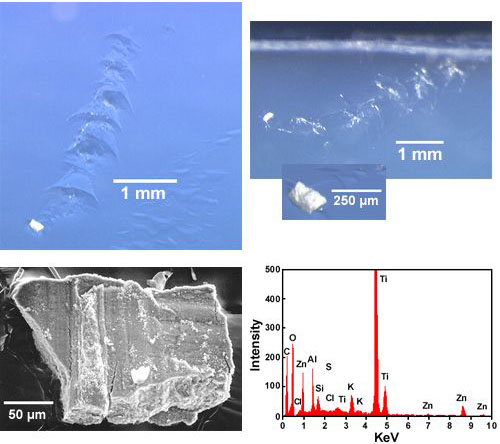
\includegraphics[width=6cm]{images/paintflakes}
  \caption{NASA, Paint flakes captured by Mir Environmental Effects Payload.}
  \label{fig:paintflakes}
\end{figure}
	
	Hypervelocity collisions of small debris objects create particles upon impact which are called ejecta and are part of the fragmentation debris group. Figure \ref{fig:hypervelocitycollision} shows a hypervelocity impact which created a hole in a panel of the Solar Maximum Mission satellite.
	
\begin{figure}[H]
\centering
  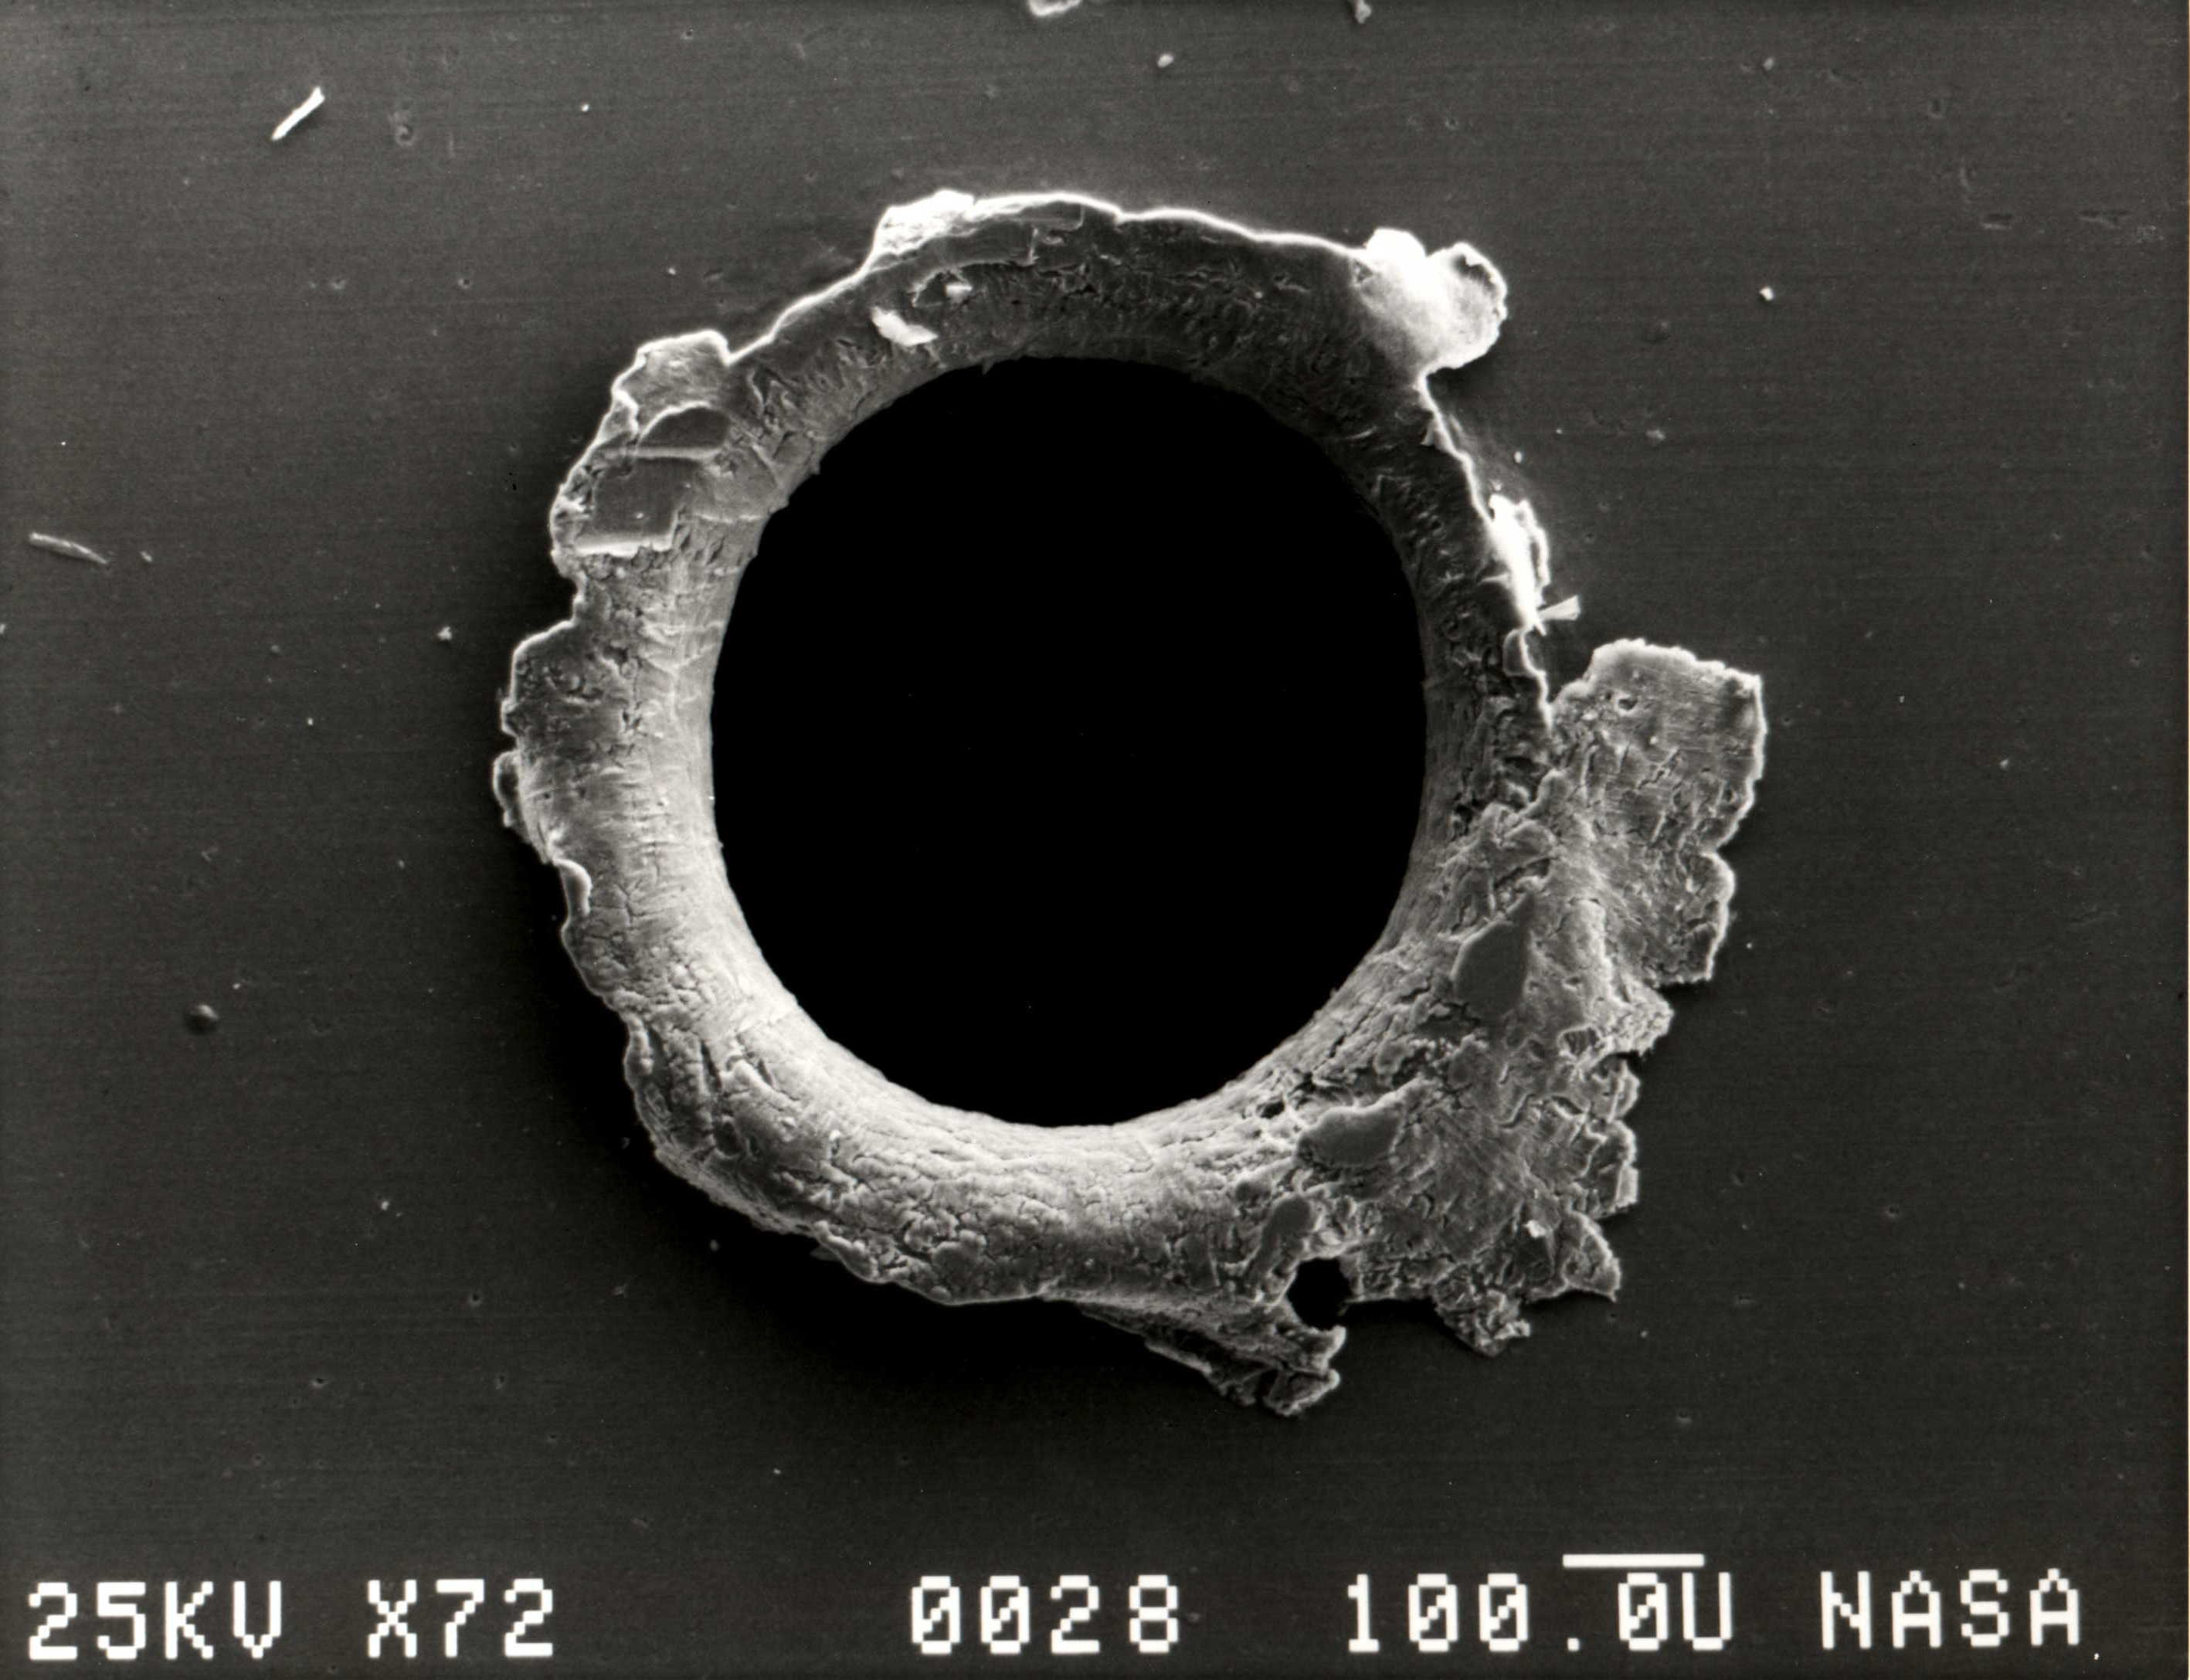
\includegraphics[width=6cm]{images/hypervelocitycollision}
  \caption{NASA, A hole made by debris in a solar panel.}
  \label{fig:hypervelocitycollision}
\end{figure}	
	
	While delivering payloads into orbit, burning process of solid rocket motors releases particles called SRM slag and SRM dust which are classified as non-fragmentation, unintentional debris and are composed mainly of aluminium oxide. Figure \ref{fig:srmslag} shows a piece of SRM slag recovered from a test firing of a shuttle solid rocket booster.
	
\begin{figure}[H]
\centering
  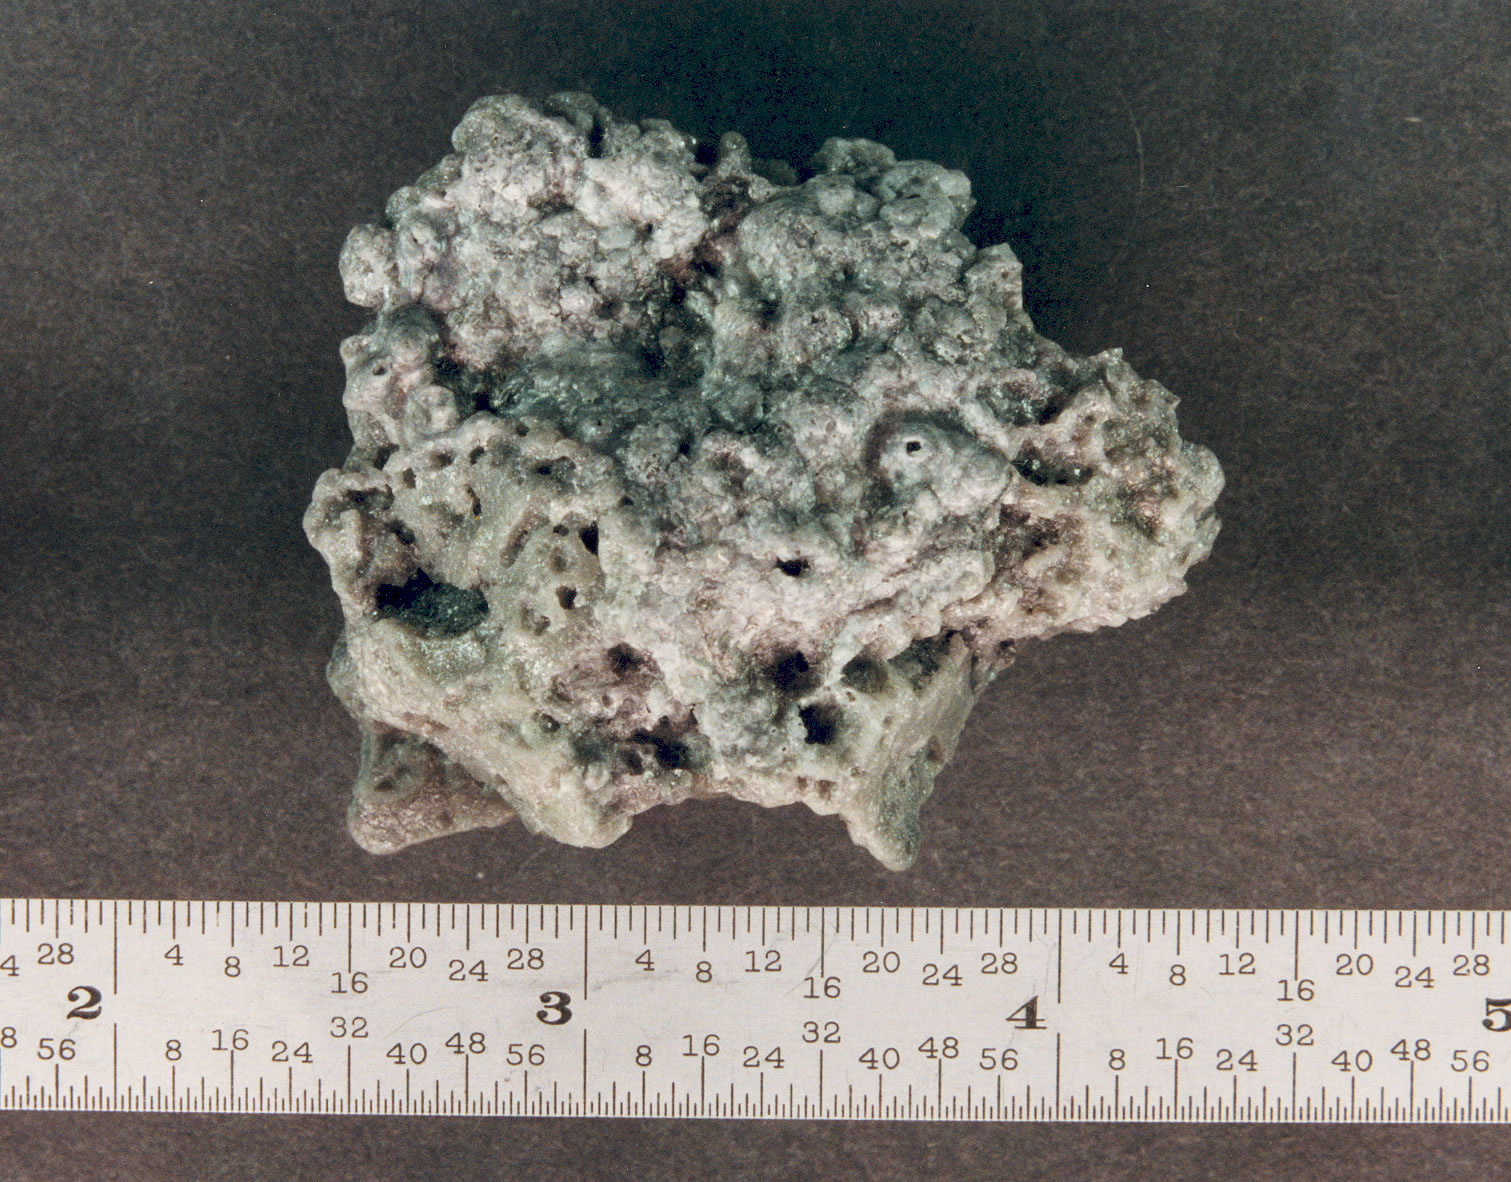
\includegraphics[width=6cm]{images/slag}
  \caption{NASA (ca. 2005), SRM slag.}
  \label{fig:srmslag}
\end{figure}	
	
	Another similar but rare type is droplets of sodium-potassium alloy (NaK), a coolant in Russian RORSAT (Radar Ocean Reconnaissance Satellites). Since this kind of reactor is no longer used, NaK droplets along with Westford Needles (see next paragraph) are considered a historic, non-reproducing space debris. 
	
	A communications experiment between years 1961 and 1963 consisted of deploying copper wires around the Earth. These copper wires were 1.78 cm long and 25.4 µm in diameter - see Figure \ref{fig:westfordneedles}. However, the deployment failed and the estimated mass of Westford Needles is less than 60 kg in two clusters.
	
\begin{figure}[H]
\centering
  
\includegraphics[width=6cm]{images/westfordneedles}
  \caption{MIT (1963), Westford needles.}
  \label{fig:westfordneedles}
\end{figure}	
	
	While being the major contributor to the population of space debris, small objects are, as mentioned, virtually unobservable from the ground, only by radars and space-based telescopes positioned on LEO, and therefore are not the main focus of this thesis. For further information see \citep{klinkrad2006space} or \citep{Silha2012id}.

\subsection{Large space debris}\label{subsec:large_space_debris}

	The most extensive database of tracked objects in orbit is maintained by US Space Surveillance Network (USSSN). Only objects which exceed certain sizes at certain altitudes can be tracked with ground-based radar and optical measurements. Due to this, USSSN incorporates only debris larger than 5 cm to 10 cm in LEO and 30 cm to 20 m in GEO (geostationary altitudes, approximately 36,000 km). Currently, USSSN contains more than 42,000 tracked objects with more than half of them still in orbit. About 24\% of them are satellites and 18\% are spent upper stages and other mission-related objects \citep{esabr336}. Out of 175 fragmentation events recorded since 1961 until January 2002, 48 have been categorized as deliberate explosions or collisions, 52 as propulsion system explosions, 10 have been caused by aerodynamic forces, 7 are believed to have been electrical system failures and 1 was an accidental collision \citep{klinkrad2006space}. 

	Deliberate collisions have been caused mainly as test scenarios for Strategic Defence Initiative (SDI) experiment. In the first case, an anti-satellite missile was fired and destroyed Solwind P78-1 satellite. The second collision was between the USA-19 spacecraft and an upper stage used to bring it into the orbit. Number of fragments for both of these events was 285 and 13 respectively but as a result of natural cleaning processes or deliberate planning, from H-10 event only 33 objects were on orbit by January 2002 and from Solwind P78-1 only 2. However, the largest fragmentation event occurred in 2007 when China intentionally destroyed its non-functional weather satellite Fengyun-1C, generating more than 3,215 new fragments. 
	
	Even though unintentional collisions are rare and only 0.2\% of all catalogued objects until February 2009 have been created in this way it is expected that they will be a major cause for debris in the future. On November 13, 1986 an Ariane-1 H-10 upper stage exploded, causing a fragment cloud containing 488 catalogue entries. The first unintentional in-orbit collision came to pass 10 years later between a French satellite and the mentioned H-10 upper stage explosion fragment. The Cerise satellite was still able to function afterwards and the event caused only one new piece of catalogued debris \citep{Silha2012id}. 
	
	A particularly interesting class of space debris is anomalous debris. It's a specific group that has small velocity and high area to mass ratio (A/M) and its formation process is unknown. The exemplary member of anomalous debris is multilayer insulation (MLI),  paint flakes and defunct solar panels. MLI is used as thermal protection to decrease thermal noise on antennae and satellite buses of spacecrafts. MLI can be divided into two types based on their purpose – as a cover/outer layer, and as a reflector/inner layer.
	
	The rapid creation of new debris of non-negligible sizes is a major concern due to the phenomenon called “Kessler syndrome”. The term was coined in 1978 and it means that “each collision would produce several hundred objects large enough to catalogue, increasing the rate that future collision breakups would occur, resulting in an exponential growth in the collision rate and debris population” (Kessler, 2009).
	
	Spent upper stages and non-functional satellites are one of the largest and most compact space debris. Even though many of them re-enter the Earth's atmosphere on purpose, or are elevated on further orbits, and thus their life on orbit is relatively short, they still pose a threat to functional satellites or missions in progress. Figure \ref{fig:upperstage} shows such spent upper stage, specifically Agena D, in the past the most launched American upper stage.
	
\begin{figure}[H]
\centering
  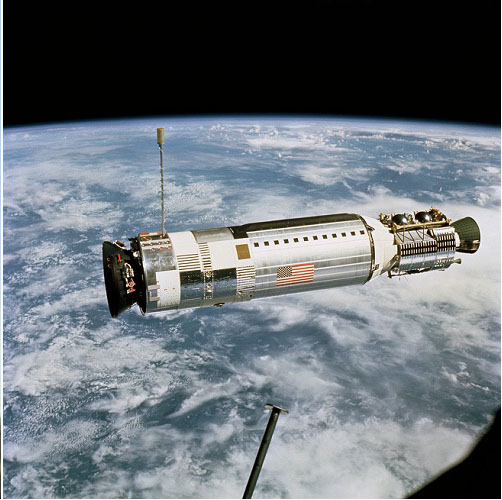
\includegraphics[width=6cm]{images/upperstage}
  \caption{NASA, Agena D upper stage.}
  \label{fig:upperstage}
\end{figure}
	
\pagebreak


\section{Observations and telescopes}\label{sec:observations_telescopes}

Optical telescopes are usually placed at high altitudes, with minimal light pollution and good meteorological and atmospheric conditions. Telescopes used for satellite tracking must be operated at "astronomical night" (Sun being more than 18° under the horizon) while the tracked objects must still be illuminated by the Sun \citep{klinkrad2006space}.

	Telescopes are divided into two groups: refractors and reflectors. The first type uses lens systems to observe objects while the second one uses mirror surfaces to focus incoming light. Reflectors are categorized into four subgroups:
	
\begin{enumerate}
	\item Newton telescopes,
	\item Cassegrain telescopes,
	\item Coudé telescopes,
	\item Ritchey-Chrétien telescopes.
\end{enumerate}
	
	The base upon which a telescope is placed is called a mount. As with telescopes, there are many types of mounts with each giving different advantages than the other. Mounts are able to rotate both vertically and horizontally \citep{klinkrad2006space}.
	
	A telescope collects photons which are reflected or emitted by a space object. Usually, the origin of photons is the Sun and depending on the angle between the Sun, the reflection efficiency of the target is determined. The light is then translated into an image which can be used to generate an exposure on an Charge-Coupled device (CCD). CCDs are photosensitive and solid-state imaging sensors which convert incoming photons into electric charges on an array of photodetectors. The time-tagged information coming from the photodetectors can be reconstructed into an image with a varying resolution. CCDs naturally heat up and the danger of thermal noise corruption is to a degree mitigated by using active coolants, such as liquid nitrogen \citep{klinkrad2006space}.

\subsection{ESA OGS}\label{subsec:esa_ogs}
European Space Agency (ESA) Optical Ground Station (OGS) is a Zeiss telescope built in the Teide Observatory, in Tenerife, Spain, 2,400 m above sea level. It's a one metre telescope with focal length 13.3 m originally used for tests with laser link, space debris observation and other astronomical night observations. The CCD camera has a field of $4000 x 4000$ pixels. The telescope can detect and track near-GEO objects down to 10-15 cm in size. Throughout years 2009 to 2013 the telescope has been credited by Minor Planet Center (MPC) with discovery of 38 minor planets.

	Figure \ref{fig:esaogs1} shows the schematic of ESA OGS. One of the most important parts is the Cassegrain focus where the CCD camera is used for observation of asteroids and for long-term monitoring of comets.


\begin{figure}[H]
\centering
  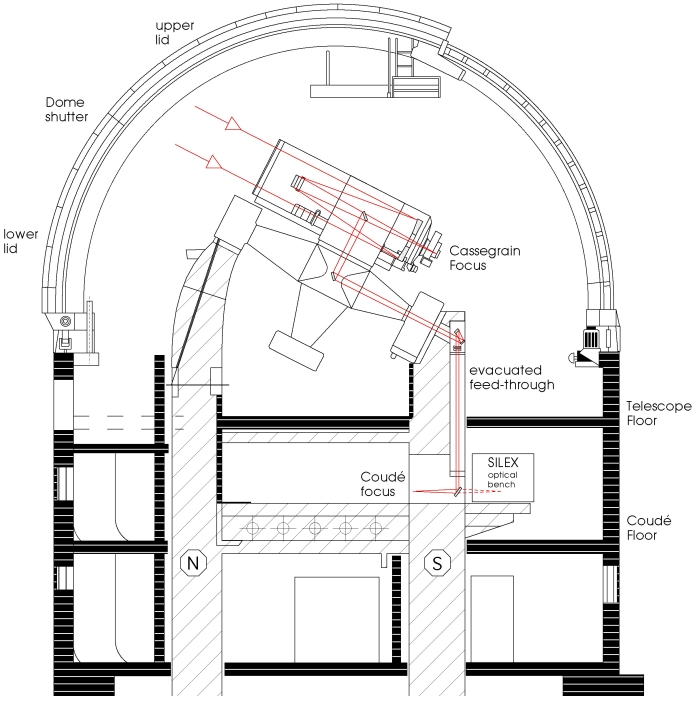
\includegraphics[width=6cm]{images/ESAOGS1}
  \caption{ESA, ESA OGS schematic.}
  \label{fig:esaogs1}
\end{figure}

	Figure \ref{fig:esaogs2} is an image of the Zeiss telescope on an English mount.

\begin{figure}[H]
\centering
  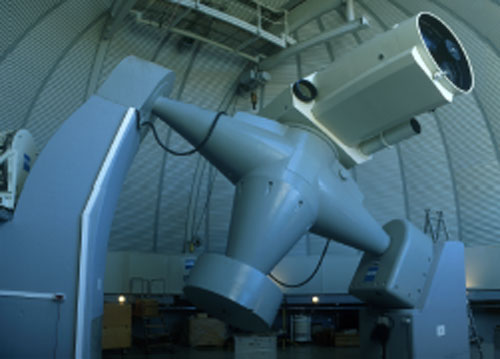
\includegraphics[width=6cm]{images/ESAOGS2}
  \caption{ESA, ESA OGS telescope.}
  \label{fig:esaogs2}
\end{figure}

\subsection{FMPI AGO}\label{subsec:fmpi_ago}
Astronomické a geofyzikálne observatórium (Astronomical and geophysical observatory, or AGO) is located in Modra, Slovakia and belongs to Fakulta matematiky, fyziky a informatiky (Faculty of mathematics, physics and informatics of Comenius University, or FMPI). The observatory has a main reflector telescope with a 0.7m Newton design Zeiss telescope with focal length of 2.961m, field of view of $28.5 x 28.5$ arc-min on an Equatorial mount. The CCD camera has resolution of $1024 x 1024$ pixels.

	Figure \ref{fig:fmpiago1} shows the schematic of the main reflector telescope and its position at AGO observatory.
	
\begin{figure}[H]
  \centering
  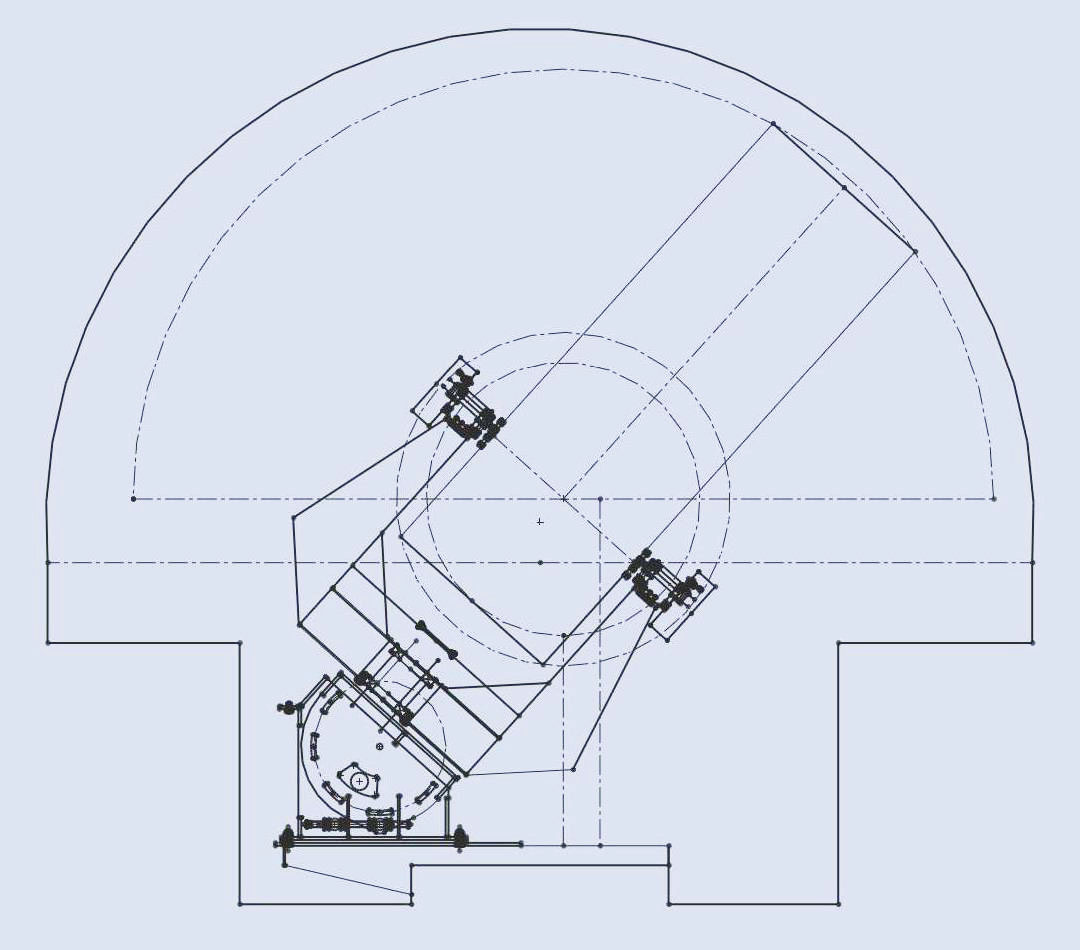
\includegraphics[width=6cm]{images/FMPIAGO1}
  \caption{KAFZM FMFI UK, Telescope schematic.}
  \label{fig:fmpiago1}
\end{figure}

	Figure \ref{fig:fmpiago2} shows the main telescope which is operated by a computer in the small AGO cupola.

\begin{figure}[H]
\centering
  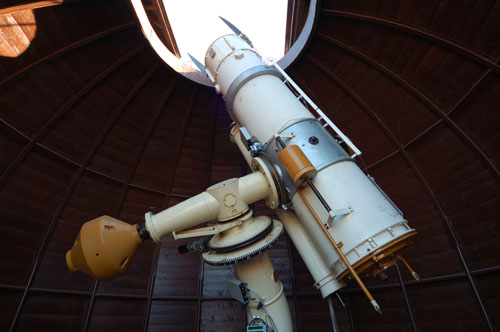
\includegraphics[width=6cm]{images/FMPIAGO2}
  \caption{KAFZM FMFI UK, The main Zeiss telescope.}
  \label{fig:fmpiago2}
\end{figure}